%  -----------------------------------------------------------------------
% |                Modelo de documento Latex para TCC do                  |
% |     curso de Engenharia da Computação da Universidade Positivo        |
%  -----------------------------------------------------------------------
% |     Produção: Eduardo J Alberti      Revisão: Veronica I. Quandt      |
%  -----------------------------------------------------------------------
% |                             Versão 2.0                                |
%  -----------------------------------------------------------------------

\documentclass{TCC_UP}

%  -----------------------------------------------------------------------
% |                 Informações para construção da Capa                   |
% |           Título, Autores, Orientador, Universidade e Ano             |
%  -----------------------------------------------------------------------

\titulo{Técnicas de Compressão de Dados em Dispositivos IoT \\ com Recursos Limitados}
    \tipotrabalho{Monografia }
    %\TipoPesquisa % Descomentar essa linha para projetos de Pesquisa

\autor{Edimar Calebe Castanho}
    \curso{Engenharia da Computação }
    \escola{Escola Politécnica }

\orientador{Julio Cesar Paes}
%\coorientador{Nome do Coorientador} % Descomentar se necessário

\makeatletter
\hypersetup{pdftitle={\@title}, pdfauthor={\@author},
            pdfsubject={\imprimirpreambulo},
            pdfkeywords={\imprimircurso}{\imprimirinstituicao}{TCC}, colorlinks=false,bookmarksdepth=4}
\makeatother
\makeindex

\begin{document}
    \pretextual
    \selectlanguage{brazil}
    \frenchspacing

%  -----------------------------------------------------------------------
% |                 Imprime a Capa e a Folha de Rosto                     |
%  -----------------------------------------------------------------------
    \imprimircapa
    \imprimirfolhaderosto

%  -----------------------------------------------------------------------
% |                       Constrói a Errata                               |
%  -----------------------------------------------------------------------
% | A errata é um elemento opcional que deve ser usado apenas quando não  |
% |   houver mais possibilidade de correção de determinado fragmento de   |
% |  texto. Substitua os elementos abaixo, e descomente, caso necessário  |
%  -----------------------------------------------------------------------
%    \begin{errata}
%        FERRIGNO, C. R. A. \textbf{Tratamento de neoplasias ósseas apendiculares com reimplantação de enxerto ósseo autólogo autoclavado associado ao plasma rico em plaquetas}: estudo crítico na cirurgia de preservação de membro em cães. 2011. 128 f. Tese (Livre-Docência) - Faculdade de Medicina Veterinária e Zootecnia, Universidade de São Paulo, São Paulo, 2011.
%            \begin{table}[htb]
%                \center
%                \begin{tabular}{|p{1.4cm}|p{1cm}|p{3cm}|p{3cm}|}
%                    \hline
%                    \textbf{Folha} & \textbf{Linha} & \textbf{Onde se lê} &
%                    \textbf{Leia-se}\\
%                    \hline
%                    1 & 10 & auto-conclavo & autoconclavo\\
%                    \hline
%                \end{tabular}
%        \end{table}
%    \end{errata}

%  -----------------------------------------------------------------------
% |                          Folha de Aprovação                           |
%  -----------------------------------------------------------------------
% | Na versão final do trabalho, a ser entregue correção de considerações |
% |  da banca de avaliação, será necessário incluir a Folha de Aprovação. |
% |   A Folha de Aprovação será cedida pela coordenação de TCC e poderá   |
% |               ser incluída por meio do comando abaixo.                |
%  -----------------------------------------------------------------------
    % \includepdf{Folha_de_Aprovacao.pdf}

%  -----------------------------------------------------------------------
% |                        Elementos Opcionais                            |
%  -----------------------------------------------------------------------
%  ------------------------- Dedicatória ---------------------------------
%    \begin{dedicatoria}
%       \vspace*{\fill}
%       \begin{adjustwidth}{9cm}{0cm}
%            Tem a finalidade de prestar homenagem a alguém e é opcional.
%       \end{adjustwidth}
%    \end{dedicatoria}
%  ----------------------- Agradecimentos --------------------------------
%    \begin{agradecimentos}
%        Os agradecimentos são opcionais e mencionam as pessoas e/ou
%        instituições que contribuíram para o desenvolvimento do trabalho.
%
%        Separe os agradecimentos em parágrafos quando o texto for longo.
%    \end{agradecimentos}
%  ------------------------- Epígrafe -----------------------------------
%    \begin{epigrafe}
%        \vspace*{\fill}
%    	\begin{adjustwidth}{9cm}{0cm}
%    		\textit{Utilizar a parte inferior da página, como neste exemplo.
%           Texto justificado e alinhado pela parte inferior da página. Em geral, contém um fragmento de texto (ex. citação curta, composição poética etc.). É relacionado ao tema ou à motivação do trabalho, e é opcional.}
%    	\end{adjustwidth}
%    \end{epigrafe}

%  -----------------------------------------------------------------------
% |                       Resumo - Obrigatório                            |
%  -----------------------------------------------------------------------
    \setlength{\absparsep}{18pt}
    \begin{resumo}
        Com o crescente uso de dispositivos IoT (Internet das Coisas) em diversas aplicações, torna-se crucial abordar os desafios associados ao armazenamento e transmissão de dados em dispositivos com recursos limitados. Este trabalho apresenta uma revisão da literatura das técnicas de compressão de dados mais relevantes para dispositivos IoT com restrições de armazenamento e largura de banda. Além disso, são discutidos estudos de caso e resultados obtidos para avaliar a eficácia dessas técnicas em cenários práticos.

        \textbf{Palavras-chave}: IoT, armazenamento, dados
    \end{resumo}

%  -----------------------------------------------------------------------
% |                       Abstract - Obrigatório                          |
%  -----------------------------------------------------------------------
    \begin{resumo}[Abstract]
     \begin{otherlanguage*}{english}
With the increasing use of IoT (Internet of Things) devices in various applications, it becomes crucial to address the challenges associated with storing and transmitting data on devices with limited resources. This work presents a literature review of the most relevant data compression techniques for IoT devices with storage and bandwidth constraints. In addition, case studies and results obtained are discussed to evaluate the effectiveness of these techniques in practical scenarios.
       \textbf{Keywords}: IoT. Storage. data.
     \end{otherlanguage*}
    \end{resumo}

%  -----------------------------------------------------------------------
% |                         Listas Opcionais                              |
%  -----------------------------------------------------------------------
%  ------------------------ Lista de Figuras -----------------------------
    \pdfbookmark[0]{\listfigurename}{lof}
    \listoffigures*
    \cleardoublepage

%  ----------------------- Lista de Gráficos -----------------------------
    \pdfbookmark[0]{\listofgraficosname}{los}
    \listofgraficos*
    \cleardoublepage

%  ------------------------ Lista de Quadros -----------------------------
    \pdfbookmark[0]{\listofquadrosname}{loq}
    \listofquadros*
    \cleardoublepage

%  ------------------------ Lista de Tabelas -----------------------------
    \pdfbookmark[0]{\listtablename}{lot}
    \listoftables*
    \cleardoublepage

%  ------------------ Lista de Abreviaturas e Siglas ---------------------
%  ------------ Utilize \nomenclature{Sigla}{Definição} ------------------
    \pdfbookmark[0]{\nomname}{las}
    \printnomenclature
    \cleardoublepage

%  ------------------------ Lista de Símbolos ----------------------------
%  ----------- Note que esta lista deve ser criada manualmente -----------
    \begin{simbolos}
      \item[$ \Omega $] Ohm
      \item[$ \Delta V $] Variação de tensão
    \end{simbolos}

%  -----------------------------------------------------------------------
% |                           Cria Sumário                                |
%  -----------------------------------------------------------------------
    \tableofcontents*
    \cleardoublepage

%  -----------------------------------------------------------------------
% |                   Inclui os arquivos de capítulos                     |
%  -----------------------------------------------------------------------
    \textual
    \pagestyle{simple}

% Inclusão de capítulos. Altera componentes de acordo com Tipo do Trabalho
    \chapter{Introdução}
\label{cap:introducao}

A Internet das Coisas (IoT) tem revolucionado a forma como interagimos com o ambiente ao nosso redor, conectando dispositivos, sensores e sistemas a uma rede global, permitindo a coleta e troca de informações em tempo real. Esta evolução tecnológica tem encontrado aplicações em diversos setores, desde a automação residencial até a otimização de processos industriais e sistemas de saúde avançados. No entanto, à medida que a IoT se expande, torna-se cada vez mais evidente a necessidade de enfrentar os desafios associados ao armazenamento e transmissão de dados em dispositivos com recursos limitados.

\section{Problema}
\label{sec:problema}

O advento da Internet das Coisas (IoT) revolucionou a forma como interagimos com o mundo ao nosso redor, conectando dispositivos, sensores e sistemas a uma rede global. No entanto, esse crescimento exponencial de dispositivos IoT trouxe consigo desafios significativos relacionados ao armazenamento e transmissão eficiente de dados. Muitos dispositivos IoT são caracterizados por recursos limitados, incluindo capacidade de armazenamento, capacidade de processamento e largura de banda de transmissão. Este cenário levanta a seguinte questão fundamental: como gerenciar eficazmente os dados gerados por dispositivos IoT em um ambiente de recursos limitados?

\section{Justificativa}
\label{sec:justificativa}

A justificativa para a realização deste trabalho reside na necessidade premente de abordar os desafios inerentes à IoT, particularmente no que diz respeito ao gerenciamento eficiente de dados em dispositivos com recursos limitados. Dispositivos IoT são amplamente utilizados em diversas aplicações, incluindo saúde, agricultura, manufatura e cidades inteligentes, e o volume de dados gerados por esses dispositivos continua a crescer exponencialmente. A compressão de dados surge como uma estratégia crucial para otimizar a utilização de recursos, economizar energia e melhorar a eficiência na transmissão de dados em redes com baixa taxa de transferência. Portanto, este trabalho se justifica pela necessidade de explorar e avaliar as técnicas de compressão de dados mais apropriadas para dispositivos IoT com recursos limitados, contribuindo para a resolução deste desafio tecnológico.

\section{Objetivo Geral}
\label{sec:ObjGeral}

O objetivo geral deste trabalho é investigar e analisar as técnicas de compressão de dados mais adequadas para dispositivos IoT com recursos limitados de armazenamento e transmissão. Isso envolve a compreensão das diferentes abordagens de compressão disponíveis, suas vantagens, desvantagens e áreas de aplicação ideais em contextos de IoT. Além disso, o objetivo geral inclui a realização de estudos de caso práticos para avaliar a eficácia dessas técnicas em cenários reais de implementação de dispositivos IoT.

\section{Objetivos Específicos}
\label{sec:ObjEspecificos}

Para atingir o objetivo geral, os seguintes objetivos específicos foram estabelecidos:

\begin{itemize}
\item Realizar uma revisão abrangente da literatura existente sobre técnicas de compressão de dados, com foco nas estratégias desenvolvidas para dispositivos IoT com recursos limitados.
\item Comparar as técnicas de compressão de dados sem perdas e com perdas, identificando suas características, vantagens e limitações.
\item Implementar um estudo de caso prático que envolva a coleta de dados por dispositivos IoT em um ambiente controlado.
\item Aplicar diversas técnicas de compressão de dados aos dados coletados e analisar os resultados em termos de economia de recursos, qualidade dos dados e eficiência da transmissão.
\end{itemize}

    \chapter{Revisão Bibliográfica}
\label{cap:revisao}

Os autores deverão, nesta seção, compor uma revisão teórica que explicite o contexto de inserção do problema levantado pelo seu projeto e dos temas principais para sua completa compreensão. 

Deve-se observar que assuntos técnicos devem ser trabalhos com cuidado para trazer informações pertinentes, relevantes e novas. Não serão aceitas revisões que descrevam o funcionamento básico de componentes eletrônicos, algoritmos ou \textit{frameworks}.

Neste sentido, pergunte-se, essa informação é relevante para compreender de forma completa o contexto no qual meu projeto está inserido? 

Exemplo -> \textit{Tema principal do trabalho:} Construção de um dispositivo capaz de identificar arritmias cardíacas. \textit{Exemplo de temas importantes a serem abordados na revisão:} o que são arritmias, quais são os tipos de arritmias cardíacas, como surgem, quais são suas consequências e formas de tratamento; efeito da doença a longo prazo, impactos sobre o sistema de saúde, dispositivos de prevenção, monitoramento e tratamento.

\textit{A organização das subseções é livre ao autor.}

\section{Trabalhos relacionados}
\label{sec:TrabalhosRelacionados}

Nesta seção, os autores deverão compor uma revisão sistemática a respeito de trabalhos relacionados ao apresentado pelo projeto.

Lembre-se de construir um comparativo através de pontos comuns entre os trabalhos e não simplesmente um resumo dos projetos analisados. 

\textit{A organização das subseções é livre ao autor.}

    \ifx\Pesquisa\undefined
        \chapter{Especificação Técnica}
\label{cap:especificacao}

\section{Análise de Contexto}
\label{sec:analiseContexto}

\subsection{Visão Geral}

Este item deverá versar \underline{obrigatoriamente} sobre o Funcionamento do Sistema e o Interfaceamento entre as partes. Descreva a visão sobre “o que” seu dispositivo ou \textit{software} fará. A organização em subseções é livre ao autor.

Para descrever claramente a visão geral é útil a utilização de diagramas em blocos, inclusive para apresentar o interfaceamento entre as partes. 

\subsection{Condições Restritivas}

Este item deverá versar \underline{obrigatoriamente}, de acordo com a aplicação no trabalho, sobre as seguintes condições restritivas

\subsubsection{Custos}

Versar sobre a existência de alguma restrição de custo. O protótipo será de baixo custo? Existe um limite de orçamento? Em uma visão de futuro, seu produto deve seguir alguma restrição de custo de operação ou de aquisição?

\subsubsection{Físicas e Ambientais}

Existe alguma restrição de funcionamento do protótipo considerando interferências físicas ou ambientais? Sua composição deve atender requisitos mínimos exigidos por alguma característica física ou ambiental de sua aplicação?

\subsubsection{Tecnológicas}

O acesso à tecnologia, ou dificuldade de acesso, pode restringir sua utilização no projeto? Existem aspectos de projeto que exigem ou impeçam a utilização de alguma tecnologia específica?

\subsubsection{Energização}
Existe alguma condição de energização do protótipo que restringe o uso de alguma tecnologia? 

\subsubsection{Interferências devido ao meio}

Existe alguma interferência devido ao meio que trará alguma restrição ao funcionamento do protótipo?

\subsection{Benefícios e Impactos}

Este item deverá versar \underline{obrigatoriamente}, de acordo com a aplicação no trabalho, sobre os seguintes benefícios e impactos

\subsubsection{Econômicos}

A implantação gerará custos ou lucros? Seu protótipo gerará economia de insumos ou outros benefícios?

\subsubsection{Operacionais}

Quais serão os prós e contras da operacionalização do projeto? Será necessário mudar a rotina do ambiente em que seu protótipo será aplicado? As mudanças impactarão positiva ou negativamente?

\subsubsection{Estratégicos}

A implantação do seu protótipo exigirá estratégias de curto ou longo prazo? A implantação do seu protótipo faz parte da estratégia de solução do problema e está relacionada a alguma outra ação? 

\subsubsection{Políticos}

Será necessário compor novas políticas públicas para implantação do seu protótipo? Seu protótipo poderá promover mudanças de aspecto legal em algum setor?

\subsubsection{Sociais}
Quais serão os benefícios ou impactos sentidos pela população ou meio-ambiente a partir da implementação do seu protótipo?

\section{Análise Funcional e de Requisitos Tecnológicos}
\label{sec:analisefuncional}

A análise funcional descreve aspectos relacionados ao funcionamento do sistema. A análise de requisitos tecnológicos nomeia as tecnologias que serão utilizadas para a construção do protótipo. Aqui também podem ser utilizadas diagramas em blocos para ilustrar a descrição (que deve ser completa).

\subsection{Lista de Funcionalidade e Atores}

Descrever em uma lista de funcionalidades que permita compreender como o sistema funcionará. Os atores do sistema deverão ser listados aqui também. Atores são todos aqueles que interagem com o sistema e que não fazem parte dele.

\subsection{Comunicação}
Como funciona toda a comunicação interna e externa do protótipo? Quais serão as tecnologias utilizadas para tal?

\subsection{Processamento}

Como será feito o processamento do protótipo? Quais serão as tecnologias utilizadas para tal? Descreva os requisitos mínimos necessários (HW e SW) para processamento das informações e ações.

\subsection{Interface Homem-Máquina}

Como será a interface do protótipo com o usuário? São utilizadas telas? Aqui devem ser mostrados protótipos das telas também.

\subsection{Sistemas Controlados Automaticamente}

O protótipo poderá processar e executar ações automaticamente? Como será feito esse processo? Existe alguma decisão que o sistema tomará sozinho?

\subsection{Aquisição de dados e Atuação}

Como e quando será feita alguma aquisição de dados? Qual será a forma de atuação do sistema em cada caso?

\section{Análise da Arquitetura do Sistema}

\subsection{Hardware}

Este item deverá versar sobre o funcionamento do dispositivo de \textit{hardware} e suas circuitarias. \underline{obrigatoriamente} os autores devem incorporar ao texto Diagramas de Blocos para a descrição do funcionamento do \textit{hardware} e a interconexão de dispositivos, bem como Diagramas de Fluxo para a descrição lógica do \textit{firmware}.

\subsection{Software}

Este item deverá versar sobre o funcionamento do \textit{software} e suas dependências. obrigatoriamente os autores deverão incorporar ao texto, por meio de seções específicas, Modelo Entidade Relacionamento (MER), Diagrama Entidade Relacionamento (DER), Use Cases, Diagramas de Sequência e Diagramas de Classe.

    \else
        \chapter{Metodologia de Pesquisa}
\label{cap:metodologia}

\section{Tipo e Objeto de Pesquisa}
\label{sec:tipo_e_Obj}

Informar o tipo da pesquisa: qualitativa, quantitativa ou qualiquantitativa. A pesquisa científica também pode ser classificada como: pesquisa bibliográfica, estudo de caso, pesquisa de campo, entre outras. Informar o objeto de pesquisa, o qual consiste no foco ou eixo central do estudo.

\section{População ou Amostra de Estudo}
\label{sec:amostra}

Uma população é um conjunto de pessoas, itens ou eventos. Nem sempre é conveniente ou possível examinar todos os membros de uma população. Assim, pode-se definir uma amostra, que é um subconjunto de uma população. Descreva a população ou amostra, e informe o número de participantes da pesquisa.

\subsection{Critérios de Inclusão}

Informar como serão compostos os grupos de participantes da pesquisa.

\subsection{Critérios de Exclusão}

Informar os critérios para a não inclusão de participantes informados no item anterior, e que não atendem aos propósitos da pesquisa.

\section{Descrição do Processo de Coleta de Dados}
\label{sec:coleta}

Informar o objetivo da aquisição dos dados, por exemplo para criação de uma base de dados, para criação ou validação do protótipo. Descrever detalhadamente a metodologia para aquisição dos dados, incluindo a forma de abordagem dos participantes, bem como o método de coleta de dados (execução de uma tarefa, questionário, entrevista etc.).

\subsection{Metodologia para revisão}

\section{Descrição do Processo de Análise de Dados}
\label{sec:analise}

Descrever o método matemático e estatístico (quantitativo e/ou qualitativo) a ser utilizado para a análise dos dados coletados.

\subsection{Análise Matemática e Estatística}

\subsection{Algoritmos e Frameworks}

Informar quais algoritmos ou \textit{frameworks} que serão utilizados na pesquisa. Eles podem ser necessários para realizar a aquisição de dados, a análise dos dados ou para a construção e validação do protótipo.

\section{Descrição do Protótipo}
\label{sec:prototipo}

\subsection{Visão Geral}

Este item deverá versar \underline{obrigatoriamente} sobre o Funcionamento do Sistema e o Interfaceamento entre as partes. Descreva a visão sobre “o que” seu dispositivo ou \textit{software} fará. A organização em subseções é livre ao autor.

Para descrever claramente a visão geral é útil a utilização de diagramas em blocos, inclusive para apresentar o interfaceamento entre as partes. 

\subsection{Lista de Funcionalidade e Atores}

Descrever em uma lista de funcionalidades que permita compreender como o sistema funcionará. Os atores do sistema deverão ser listados aqui também. Atores são todos aqueles que interagem com o sistema e que não fazem parte dele.

\subsection{Comunicação}
Como funciona toda a comunicação interna e externa do protótipo? Quais serão as tecnologias utilizadas para tal?

\subsection{Processamento}

Como será feito o processamento do protótipo? Quais serão as tecnologias utilizadas para tal? Descreva os requisitos mínimos necessários (HW e SW) para processamento das informações e ações.

\subsection{Interface Homem-Máquina}

Como será a interface do protótipo com o usuário? São utilizadas telas? Aqui devem ser mostrados protótipos das telas também.

\subsection{Sistemas Controlados Automaticamente}

O protótipo poderá processar e executar ações automaticamente? Como será feito esse processo? Existe alguma decisão que o sistema tomará sozinho?

\subsection{Aquisição de dados e Atuação}

Como e quando será feita alguma aquisição de dados? Qual será a forma de atuação do sistema em cada caso?

    \fi
    \chapter{Desenvolvimento}
\label{cap:desenvolvimento}

O desenvolvimento da Ferramenta de Compressão de Dados foi um processo estruturado que seguiu etapas específicas para garantir a implementação eficiente dos algoritmos de compressão e descompressão.

\section{Planejamento e Estruturação do Projeto}

A estrutura do projeto foi delineada considerando a modularidade e a organização dos códigos-fonte. A divisão em diretórios específicos (\texttt{src}, \texttt{lib}, \texttt{bin}) permitiu uma clara separação entre o código principal, bibliotecas de terceiros e o diretório de saída para os arquivos objeto e o executável final. Isso facilitou a manutenção e compreensão do projeto.

\section{Implementação dos Algoritmos de Compressão e Descompressão}

Os algoritmos escolhidos (Huffman, Deflate, RLE e LZW) foram implementados de acordo com as especificações, garantindo sua correta funcionalidade. Cada algoritmo teve sua implementação dedicada (\texttt{huffman.c}, \texttt{deflate.c}, \texttt{rle\_routine.c}, \texttt{lzw\_compress.c}), o que permitiu a modularidade e manutenção separada de cada método.

\section{Utilização de Ferramentas de Compilação}

Para facilitar o processo de compilação e geração do executável final, foi utilizado um \texttt{Makefile}. Esse arquivo configurou os parâmetros de compilação e vinculação dos diferentes arquivos-fonte presentes nos diretórios \texttt{src} e \texttt{lib}, agilizando o processo de geração do executável final no diretório \texttt{bin}.

\section{Validação e Testes}

Durante o desenvolvimento, foram realizados testes extensivos para garantir o correto funcionamento dos algoritmos de compressão e descompressão. Esses testes foram conduzidos utilizando diferentes tipos de arquivos e dados, verificando a integridade e a eficiência dos algoritmos implementados.

\section{Documentação e Limpeza}

Além da implementação, a ferramenta foi documentada adequadamente no arquivo README.md, fornecendo instruções claras sobre a compilação, uso da ferramenta e limpeza de arquivos gerados durante o processo.

O processo de desenvolvimento foi centrado na eficiência, modularidade e facilidade de uso da Ferramenta de Compressão de Dados, garantindo a correta aplicação dos algoritmos e a entrega de uma solução funcional e bem documentada para compressão e descompressão de dados.

    \chapter{Teste e Resultados}
\label{cap:teste-resultados}

Neste capítulo, descrevemos os testes de validação realizados para a ferramenta de compressão de dados utilizando diferentes algoritmos. Estes testes foram conduzidos em dois diferentes ambientes: um processador ARMv6 com 256MB de memória RAM e um processador x86 (Ryzen 6) com 32GB de RAM. Os resultados obtidos são apresentados a seguir:

\section{Testes no Processador ARMv6}

Os testes realizados no processador ARMv6 apresentaram os seguintes resultados:

\begin{center}
\begin{tabular}{|c|c|c|c|}
\hline
Algoritmo & Operação & Tempo (s) & Tamanho do arquivo (kB) \\
\hline
Huffman & Compressão & 0.669 & 176 \\
Huffman & Descompressão & 0.098 & 688 \\
Deflate & Compressão & 0.699 & 176 \\
Deflate & Descompressão & 0.085 & 688 \\
RLE & Compressão & 0.806 & 1232 \\
RLE & Descompressão & 0.086 & 680 \\
LZW & Compressão & 40.834 & 228 \\
LZW & Descompressão & 0.146 & 688 \\
\hline
\end{tabular}
\end{center}

Os resultados obtidos no processador ARMv6 indicam tempos de processamento mais prolongados em comparação com o ambiente x86, especialmente para o algoritmo LZW.

\section{Testes no Processador x86}

Já os testes no processador x86, com um ambiente mais robusto em termos de hardware, apresentaram os seguintes resultados:

\begin{center}
\begin{tabular}{|c|c|c|c|}
\hline
Algoritmo & Operação & Tempo (s) & Tamanho do arquivo (kB) \\
\hline
Huffman & Compressão & 0.161 & 176 \\
Huffman & Descompressão & 0.008 & 688 \\
Deflate & Compressão & 0.161 & 176 \\
Deflate & Descompressão & 0.008 & 688 \\
RLE & Compressão & 0.024 & 1232 \\
RLE & Descompressão & 0.005 & 680 \\
LZW & Compressão & 3.515 & 228 \\
LZW & Descompressão & 0.011 & 688 \\
\hline
\end{tabular}
\end{center}

No ambiente x86, os tempos de processamento foram significativamente menores em comparação com o ARMv6, indicando uma melhoria considerável de desempenho, especialmente para o algoritmo LZW.

\section{Discussão dos Resultados}

Os resultados dos testes demonstram claramente a influência do hardware no desempenho da ferramenta de compressão de dados. Ambos os ambientes apresentaram variações significativas nos tempos de compressão e descompressão, destacando a importância do hardware na eficiência dos algoritmos utilizados.

Além disso, os dados obtidos fornecem informações valiosas sobre os tempos de execução dos diferentes algoritmos em diferentes ambientes, contribuindo para a compreensão do desempenho da ferramenta em contextos variados.

    \chapter{Conclusões}
\label{cap:conclusoes}

Além das conclusões pertinentes ao trabalho, os autores devem \underline{obrigatoriamente} indicar possibilidades de Trabalhos Futuros derivados do desenvolvimento de seu protótipo.
    \phantompart

%  -----------------------------------------------------------------------
% |                      Inclui elementos pós-textuais                    |
%  -----------------------------------------------------------------------
    \postextual
    \bibliography{Bibliografia}
    \begin{apendicesenv}

\chapter{Exemplo de Apêndice}
\label{cap:apendice}

    Exemplo de Apêndice. Aqui, aproveitamos para descrever a regra para inserção de Figuras. As Figuras devem ser centralizadas, com legenda e fonte descritas alinhadas à esquerda, como pode ser observado pela Figura \ref{fig:exemplo}. O mesmo ocorre para os gráficos, como apresentado pelo Gráfico \ref{fig:exgrafico}. 
    
    \begin{figure}[h]
        \caption{Exemplo de Imagem.}
        \begin{center}
            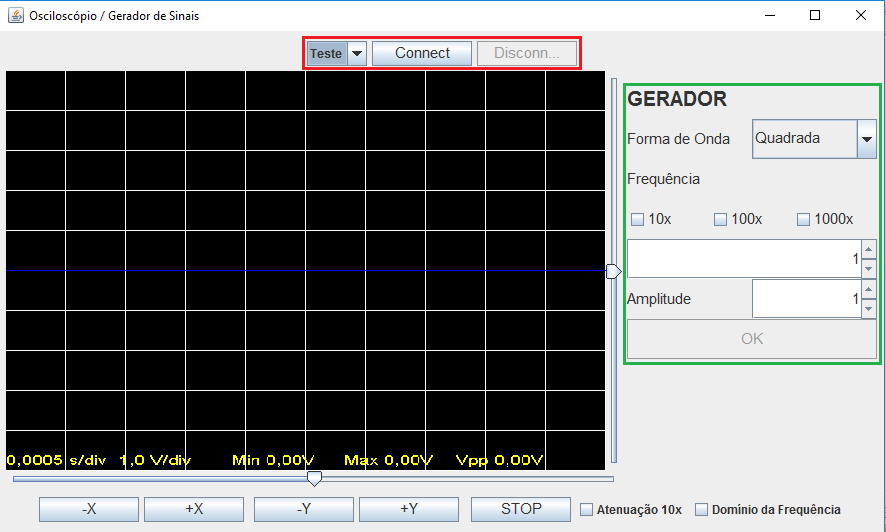
\includegraphics[width=0.6\linewidth]{Imagens/Tela.png}
        \end{center}
        \legend{\small{Fonte: \citeonline{SantanadaSilva2020}}}
        \label{fig:exemplo}
    \end{figure}
    
    \begin{grafico}[h]
        \caption{Exemplo de Gráfico.}
        \begin{center}
            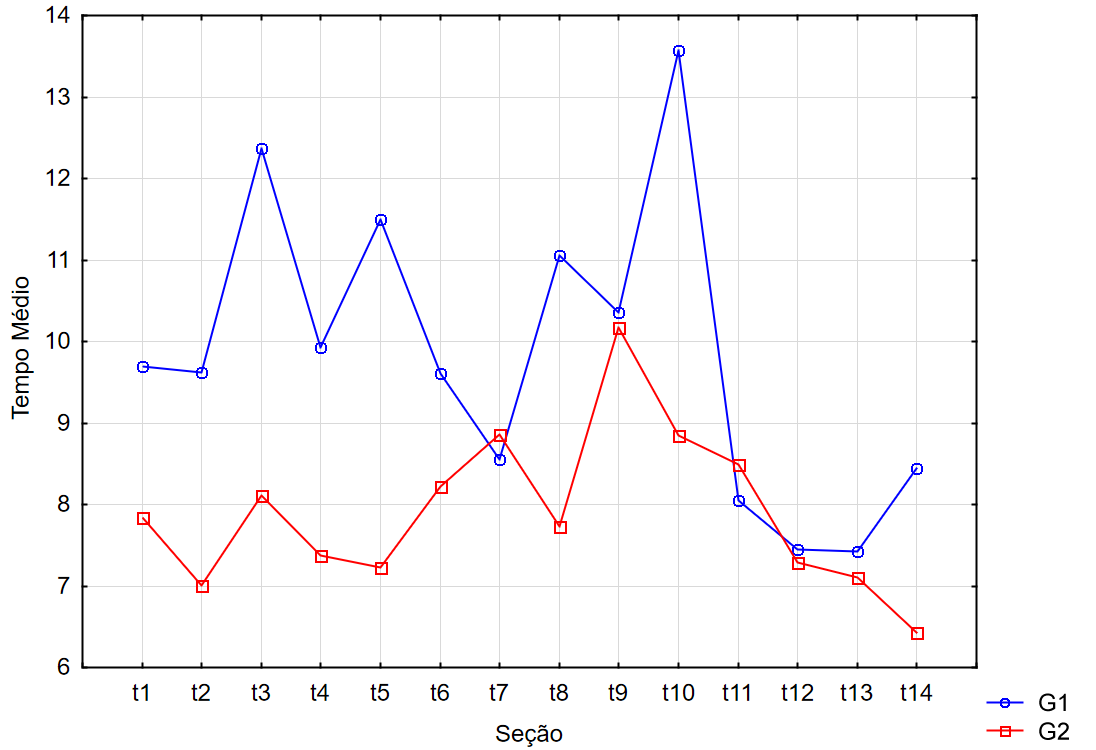
\includegraphics[width=0.6\linewidth]{Imagens/grafico.png}
        \end{center}
        \label{fig:exgrafico}
    \end{grafico}

    Ainda, tabelas que possuem apenas informações textuais, devem ser nomeadas por quadros, como apresenta o Quadro \ref{qua:exemplo}.
    
    \begin{quadro}[ht]
        \caption{Exemplo de Quadro}
        \begin{tabular}{ll}
            \toprule
            Termo & Significado \\
            \midrule
            char  & Um caractere, ou valor inteiro não sinalizado com 8 bits \\
            int   & Valor numérico com 4 bytes de comprimento \\
            \bottomrule
            \bottomrule
        \end{tabular}
        \label{qua:exemplo}
    \end{quadro}
    
\end{apendicesenv}
    \begin{anexosenv}

\chapter{Exemplo de Anexo}
\label{cap:anexo}

    Este é um exemplo de anexo. Aqui aproveitamos para apresentar a construção de tabelas. As tabelas, assim como figuras, devem ser nomeadas e conter legendas alinhadas à esquerda, como apresenta a Tabela \ref{tab:exemplo}.

\begin{table}[htbp]
  \centering
  \caption{Exemplo de tabela}
    \begin{tabular}{rrrrrr}
    \toprule
          & \multicolumn{1}{l}{Altura} & \multicolumn{1}{l}{Prop.A} & \multicolumn{1}{l}{Prop.B} & \multicolumn{1}{l}{Prop.C} & \multicolumn{1}{l}{Prop.D} \\
    \midrule
    1     & 152.3115 & -19.6 & 30.88 & 33.12 & 0 \\
    2     & 161.3583 & 20.8959 & 30.49673 & 23.39696 & 10.32693 \\
    3     & 184.5315 & 23.89683 & 34.87646 & 26.75707 & 11.81002 \\
    4     & 175.0984 & 22.67524 & 33.0936 & 25.38927 & 11.2063 \\
    5     & 187.0856 & 24.22758 & 35.35918 & 27.12741 & 11.97348 \\
    6     & 164.3629 & 21.28499 & 31.06458 & 23.83262 & 10.51922 \\
    7     & 194.6153 & 25.20268 & 36.78229 & 28.21921 & 12.45538 \\
    8     & 163.868 & 21.22091 & 30.97105 & 23.76086 & 10.48755 \\
    9     & 163.5961 & 21.1857 & 30.91966 & 23.72144 & 10.47015 \\
    10    & 195.9685 & 25.37792 & 37.03805 & 28.41543 & 12.54198 \\
    11    & 194.2495 & 25.15531 & 36.71316 & 28.16618 & 12.43197 \\
    12    & 202.0585 & 26.16658 & 38.18906 & 29.29848 & 12.93174 \\
    13    & 183.856 & 23.80935 & 34.74879 & 26.65912 & 11.76679 \\
    14    & 168.8063 & 21.86041 & 31.90439 & 24.47691 & 10.8036 \\
    15    & 180.949 & 23.4329 & 34.19936 & 26.23761 & 11.58074 \\
    16    & 169.6921 & 21.97512 & 32.0718 & 24.60535 & 10.86029 \\
    17    & 164.2326 & 21.26813 & 31.03997 & 23.81373 & 10.51089 \\
    18    & 203.7827 & 26.38986 & 38.51493 & 29.54849 & 13.04209 \\
    19    & 160.2441 & 20.75161 & 30.28614 & 23.2354 & 10.25562 \\
    20    & 164.6612 & 21.32363 & 31.12097 & 23.87588 & 10.53832 \\
    21    & 159.3832 & 20.64012 & 30.12342 & 23.11056 & 10.20052 \\
    22    & 141.8475 & 18.36925 & 26.80917 & 20.56789 & 9.078239 \\
    23    & 168.5719 & 21.83006 & 31.86009 & 24.44292 & 10.7886 \\
    24    & 183.5559 & 23.77049 & 34.69207 & 26.61561 & 11.74758 \\
    25    & 164.6031 & 21.3161 & 31.10999 & 23.86745 & 10.5346 \\
    26    & 185.039 & 23.96255 & 34.97237 & 26.83065 & 11.84249 \\
    27    & 177.4706 & 22.98245 & 33.54195 & 25.73324 & 11.35812 \\
    28    & 216.0425 & 27.97751 & 40.83204 & 31.32616 & 13.82672 \\
    29    & 195.0084 & 25.25359 & 36.85658 & 28.27622 & 12.48054 \\
    30    & 162.5406 & 21.04901 & 30.72018 & 23.56839 & 10.4026 \\
    \bottomrule
    \bottomrule
    \end{tabular}%
    \legend{\small{Os autores podem descrever Fonte ou outras informações sobre a Tabela}}
  \label{tab:exemplo}%
\end{table}%

    
\end{anexosenv}

\end{document}
